\chapter{結果}

\section{記述統計・基礎集計}
本章では、第2章で定義した新規性指標（上位$k\%$平均に基づく \texttt{change\_topk}）と、
提出日をイベント日とするイベント・スタディのアウトカム（\texttt{abvol\_mkt}, \texttt{vol\_abs}, \texttt{car\_mm}）の関係を、実証結果として整理する。

分析対象は有価証券報告書「事業等のリスク」欄であり、イベント窓は提出日周り（$-1,+1$）の反応を中心に確認する。
また、推定に用いる回帰仕様は第2章のとおり、企業の財務特性を統制し、年固定効果および業種固定効果を含める。
標準誤差は企業でクラスタ化する。

サンプルは、イベント窓の株価データおよび統制変数が揃う観測に限定されるため、回帰によって有効サンプル数が異なる。
以降では、各推定結果に併せてサンプル数$n$を明記する。

\section{主結果}
主結果として、イベント窓（$-1,+1$）で算出したアウトカムを被説明変数にとり、
新規性（\texttt{change\_topk}）の係数$\beta$を推定した。

結果として、新規性は株価の累積異常リターン（\texttt{car\_mm}）よりも、
異常出来高（\texttt{abvol\_mkt}）に対して強く正の関係を示した。
具体的には、\texttt{abvol\_mkt} を被説明変数とする回帰で $\beta=3.530$（$t=6.046,\,p<0.001,\,n=5606$）となり、
新規性の高いリスク開示ほど投資家の注目（出来高）が高まる傾向が確認された。
一方で、\texttt{car\_mm}（$\beta=0.006,\,p=0.152$）および \texttt{vol\_abs}（$\beta=0.006,\,p=0.170$）については、
同一仕様では統計的に明確な関係は確認されなかった。

\begin{figure}[t]
  \centering
  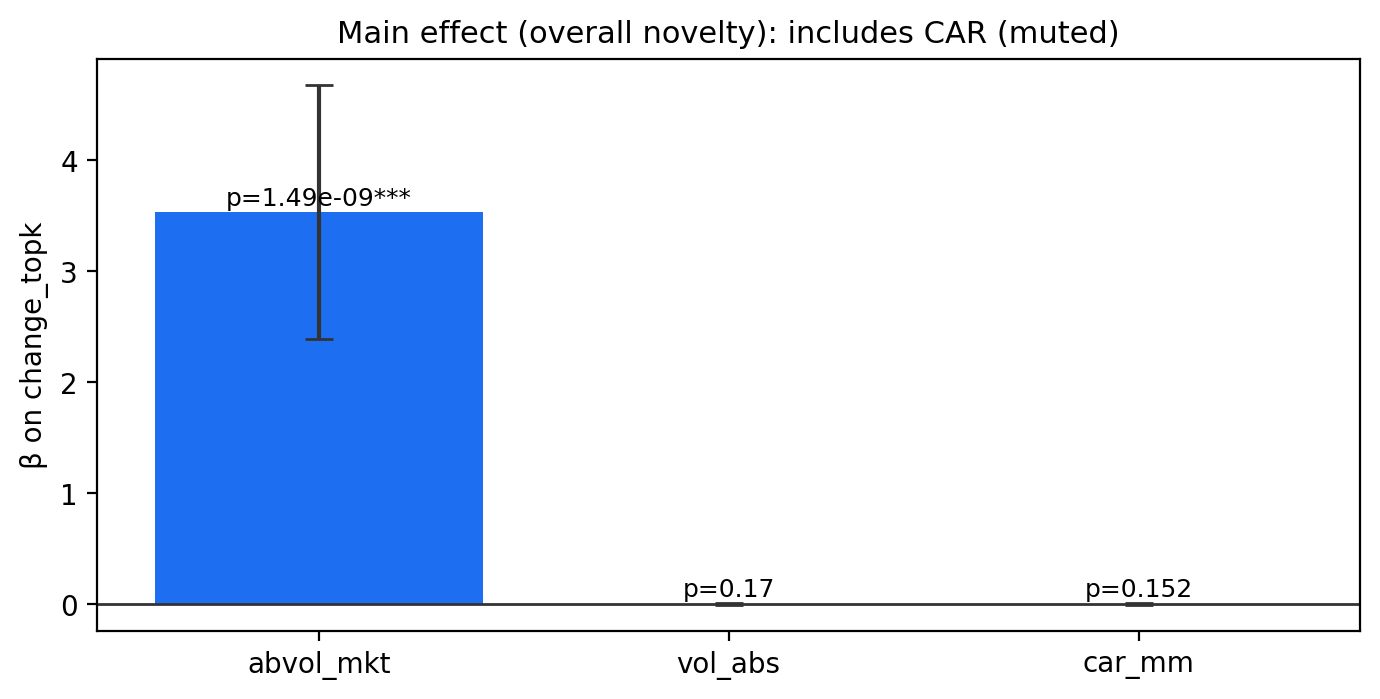
\includegraphics[width=0.92\textwidth]{figures/slide7_main_effect_ci_with_car.png}
  \caption{新規性（\texttt{change\_topk}）とイベント窓アウトカムの関係（係数と信頼区間）}
  \label{fig:main_effect_ci}
\end{figure}

\section{追加分析/頑健性確認}
本節では、（i）リスクカテゴリ別の異質性、（ii）プレトレンド、（iii）プラセボ（偽イベント日）等により、主結果の頑健性を検討する。

\subsection{カテゴリ別の異質性}
リスク文書をカテゴリ（地政学、災害/BCP、規制/コンプライアンス、人材、サイバー等）に分解し、
各カテゴリの新規性指標を用いて同様の回帰を行った。
異常出来高（\texttt{abvol\_mkt}）に対しては、災害/BCP（$\beta=2.078,\,p<0.001$）、
規制/コンプライアンス（$\beta=1.594,\,p<0.001$）、
人材（$\beta=0.807,\,p<0.01$）が正に有意であり、
新規性が注目を集める効果はカテゴリによって強弱があることが示唆される。

\begin{figure}[t]
  \centering
  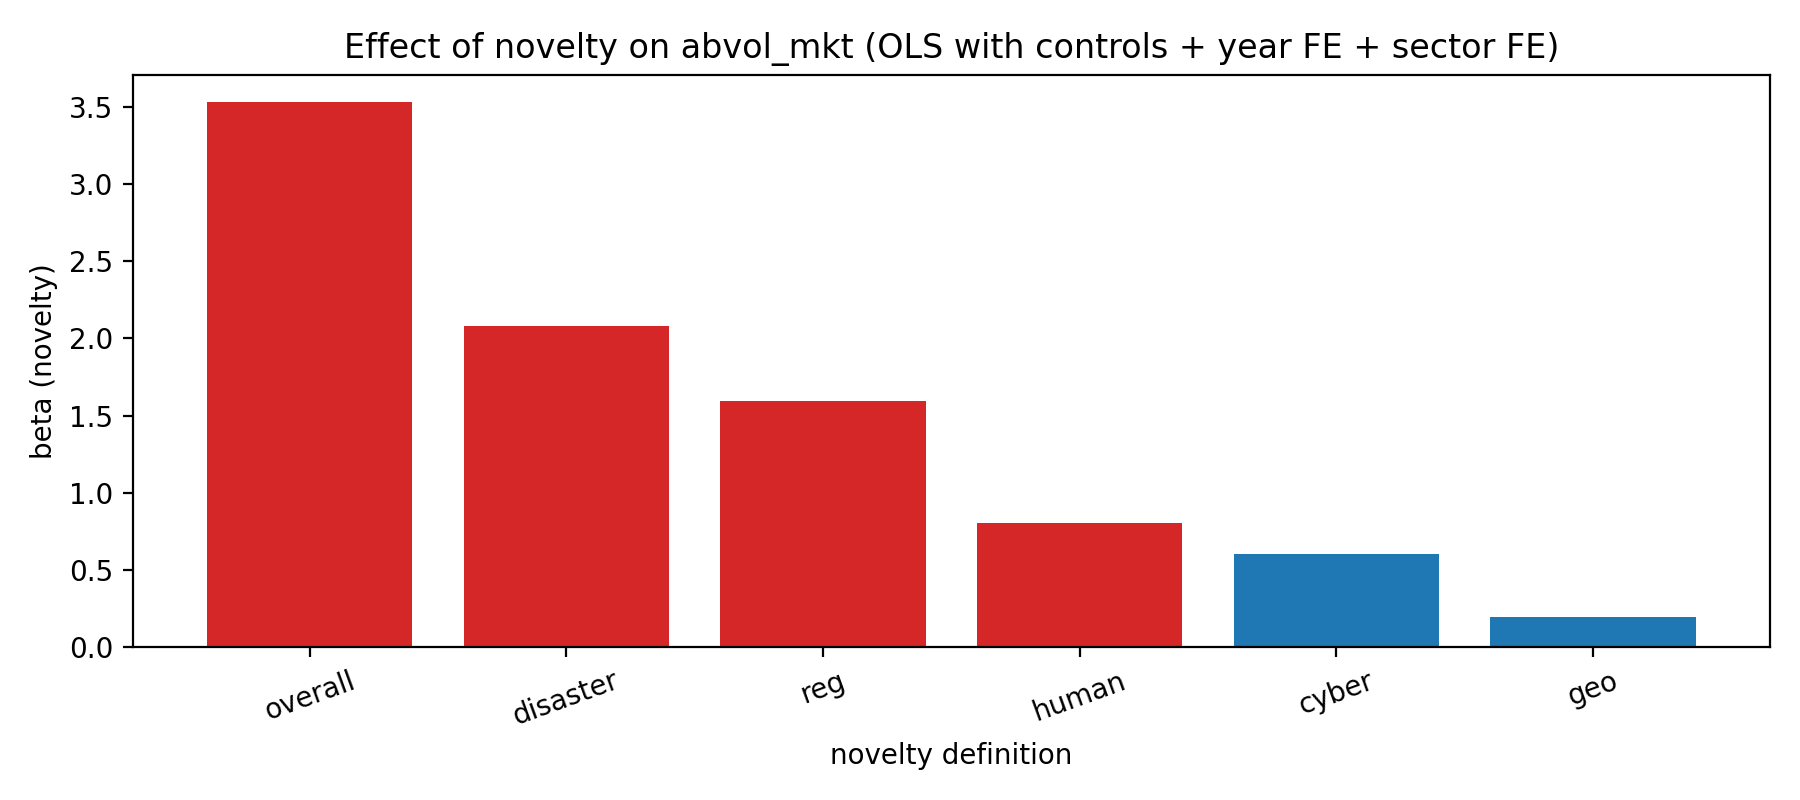
\includegraphics[width=0.92\textwidth]{figures/writeup_beta_abvol_by_category.png}
  \caption{カテゴリ別新規性と異常出来高（\texttt{abvol\_mkt}）の関係（係数と信頼区間）}
  \label{fig:abvol_by_category}
\end{figure}

\subsection{プレトレンド（事前窓）}
提出日の反応が、提出以前からのトレンド（事前窓）と区別できているかを確認するため、
事前窓（例：$-3,-1$）で算出したアウトカムと新規性の関係を推定した。
結果として、事前窓の異常出来高は新規性と強く相関し（$\beta=4.696,\,p<0.001$）、
提出日以前から注目が高い文書ほど新規性も高い可能性が示された。
この点は、新規性の解釈（情報の希少性だけでなく、企業・状況の背景要因を反映している可能性）において重要である。

\subsection{プラセボ（偽イベント日）と仕様変更}
さらに、イベント日を提出日からランダムにシフトした偽イベント日（プラセボ）を用い、
同一の推定仕様で「偽イベントでも同様の関係が出るか」を確認した。
仕様によってはプラセボ側の係数も一定の大きさを持つ場合があり、推定結果の解釈には注意が必要である。
また、企業固定効果を導入する仕様や、事前窓のアウトカムを統制変数として加える仕様では、
主結果（\texttt{abvol\_mkt} の正の関係）が弱まる傾向が確認された。

\subsection{外生ショック年ダミーを用いた追加分析}
外部イベント（ショック年）を用いた相互作用の推定も行い、
災害カテゴリ等における関係の変化を確認した。
図\ref{fig:shock_disaster}は、災害カテゴリに関する推定例を示す。

\begin{figure}[t]
  \centering
  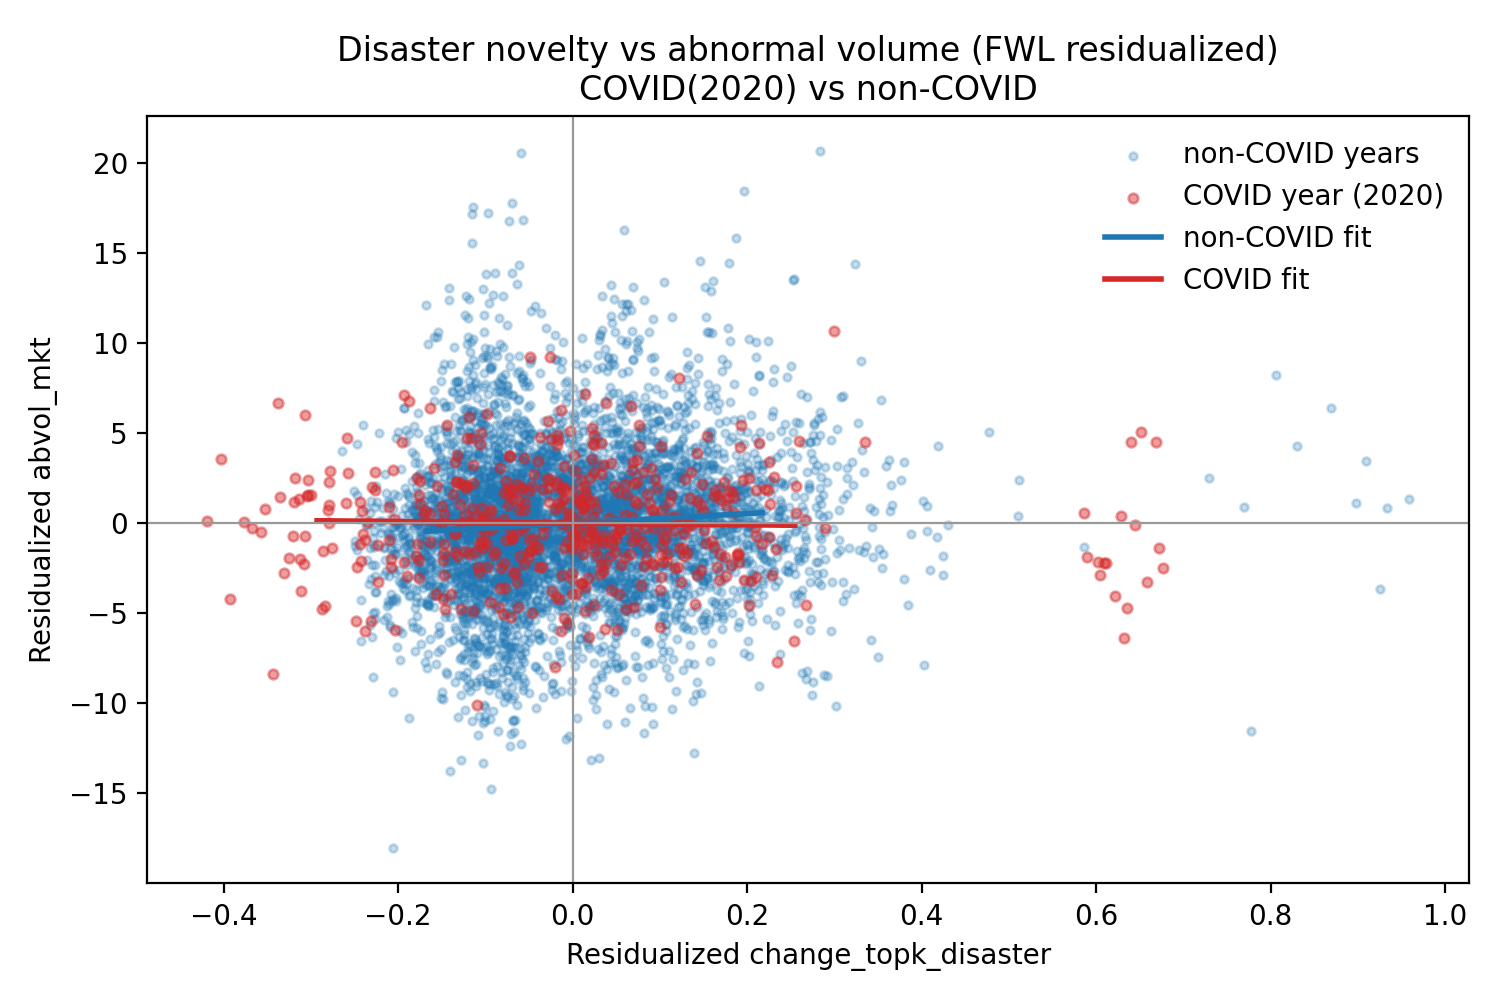
\includegraphics[width=0.92\textwidth]{figures/shock_disaster_scatter_fwl.png}\par
  \medskip
  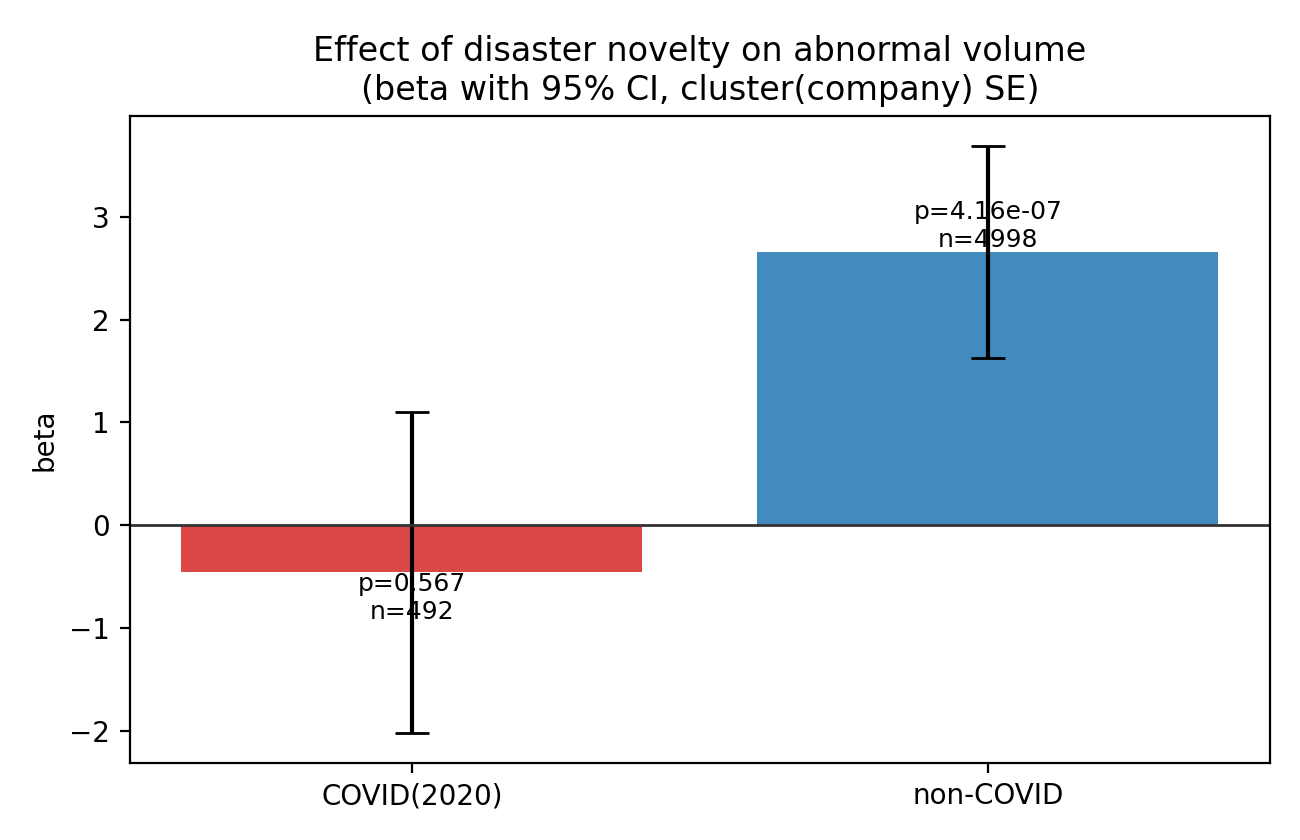
\includegraphics[width=0.92\textwidth]{figures/shock_disaster_beta_ci.png}
  \caption{外生ショック年を用いた推定例（災害カテゴリ）}
  \label{fig:shock_disaster}
\end{figure}


